\section{Theory Questions}
\label{sec:theory-questions}

\begin{problem}
  Show that if you use the line equation
  $\rho = x \cos \theta + y \sin \theta$,
  each image point $x, y$ results in a sinusoid in
  $(\rho, \theta)$ Hough space.
  Relate the amplitude and the phase of the sinusoid
  to the point $(x, y)$.
  \begin{Answer}
    For an arbitrary point $(x, y)$, its distance
    from the origin is $r = \sqrt{x^2 + y^2}$
    and the equation of the line in $(\rho, \theta)$ space
    is $\rho = x \cos \theta + y \sin \theta$.
    We can derive the equivalent sinusoid:
    \begin{align*}
      \rho &= x \cos \theta + y \sin \theta \\
      \rho &= r \left(\frac{x \cos \theta}{r} + \frac{y \sin \theta}{r} \right) \\
      \rho &= r \left(\sin \gamma \cos \theta + \cos \gamma \sin \theta \right) &\text{\zaff{ (since $x$, $y$, and $r$ form a right-angle triangle)}} \\
      \rho &= r \sin (\gamma + \theta)
    \end{align*}
    Therefore, the equivalent sinusoid has amplitude $r = \sqrt{x^2 + y^2}$
    and a phase-shift $\displaystyle \gamma = \arctan \left(\frac{x}{y} \right)$.
  \end{Answer}
\end{problem}

\newpage
\begin{problem}
  \begin{enumroman}
  \item Why do we parametrize the line in terms of $(\rho, \theta)$
  instead of the slope and the intercept, $(m, c)$?
  \begin{Answer}
    Representing the line in terms of $(\rho, \theta)$
    reduces the space of the parameters.
    In slope form ($y = mx + c$), the slope $m$ and the intercept $c$
    have a range of $[-\infty, \infty]$.
    The accumulator needed to store the votes for each possible
    line is therefore unbounded.
    In $(\rho, \theta)$ form, $\theta$ is an angle in the range
    $[0, 360]$ and $\rho$ is bounded by the longest possible distance
    in the image, $\sqrt{W^2 + H^2}$, allowing us to more feasibly
    compute the accumulator array and find lines in the image.
  \end{Answer}

  \item Express the slope and the intercept in terms of $(\rho, \theta)$.
  \begin{Answer}
    Recall that $\rho = x \cos \theta + y \sin \theta$.
    By re-arranging the equation, we get:
    \begin{multicols}{2}
      \noindent
      \begin{align*}
        x \cos \theta + y \sin \theta &= \rho \\
        y \sin \theta &= \rho - x \cos \theta \\
        y &= \frac{\rho}{\sin \theta} - \frac{\cos \theta}{\sin \theta}x
      \end{align*}
      \begin{align*}
        y &= mx + c \\
        &\implies m = - \frac{\cos \theta}{\sin \theta} = -\cot \theta \\
        &\implies c = \frac{\rho}{\sin \theta}
      \end{align*}
    \end{multicols}
  \end{Answer}
  \end{enumroman}
\end{problem}

\begin{problem}
  Assuming that the image points $(x, y)$ are in an image
  of width $W$ and height $H$,that is $x \in [1, W]$ and $y \in [1, H]$,
  what is the maximum absolute value of $\rho$,
  and what is the range of $\theta$?
  \begin{Answer}
    The maximum absolute value of $\rho$ is the longest distance
    that can fit in the image, $\sqrt{W^2 + H^2}$.

    \step
    The range of $\theta$ is $[0, 360]$.
  \end{Answer}
\end{problem}

\newpage
\begin{problem}
  For point $(10, 10)$ and points $(20, 20)$ and $(30, 30)$
  in the image, plot the corresponding sinusoid waves in Hough space
  and visualize how their intersection point defines the line.
  What is $(m, c)$ for this line?
  % \begin{Answer}
    \begin{table}[h!]
      \begin{tabular}{l | c | c | r}
        \toprule
        Point $(x, y)$ & $r = \sqrt{x^2 + y^2}$ & $\gamma = \arctan (x/y)$ & Sinusoid \\
        \midrule
        $(10, 10)$ & $\sqrt{200}$ & $45$ & $\sqrt{200}\ \sin (\theta + 45)$\\
        \midrule
        $(20, 20)$ & $\sqrt{800}$ & $45$ & $\sqrt{800}\ \sin (\theta + 45)$\\
        \midrule
        $(30, 30)$ & $\sqrt{1800}$ & $45$ & $\sqrt{1800}\ \sin (\theta + 45)$\\
        \bottomrule
      \end{tabular}
      \caption{Point and sinusoid values}
    \end{table}

    \begin{figure}[h]
      \centering
      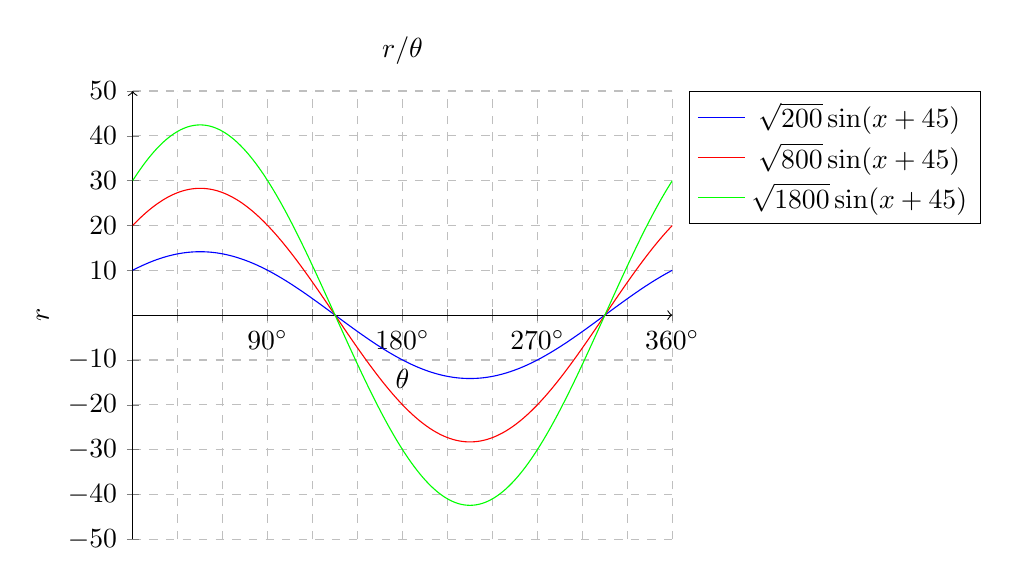
\begin{tikzpicture}
        \begin{axis}[
            title={$r/\theta$},
            axis lines=middle,
            axis line style={->},
            ylabel near ticks,
            xlabel near ticks,xlabel=$\theta$, ylabel=$r$,
            xmin=0, xmax=360, ymin=-50, ymax=50,
            xtick={0, 30, 60, 90, 120, 150, 180, 210, 240, 270, 300, 330, 360},
            ytick={-50, -40, -30, -20, -10, 0, 10, 20, 30, 40, 50},
            xticklabels={$0$, $$, $$, $90^\circ$, $$, $$, $180^\circ$, $$, $$, $270^\circ$, $$, $$, $360^\circ$},
            yticklabels={$-50$, $-40$, $-30$, $-20$, $-10$, $0$, $10$, $20$, $30$, $40$, $50$},
            grid=major, grid style=dashed,
            legend pos=outer north east % Position of the legend
          ]
            \addplot[domain=0:360, samples=360, color=blue, mark=none] {sqrt(200) * sin(x + 45)};
            \addlegendentry{$\sqrt{200} \sin(x + 45)$} % Legend entry for the first plot
            \addplot[domain=0:360, samples=360, color=red, mark=none] {sqrt(800) * sin(x + 45)};
            \addlegendentry{$\sqrt{800} \sin(x + 45)$} % Legend entry for the second plot
            \addplot[domain=0:360, samples=360, color=green, mark=none] {sqrt(1800) * sin(x + 45)};
            \addlegendentry{$\sqrt{1800} \sin(x + 45)$} % Legend entry for the third plot
        \end{axis}
    \end{tikzpicture}
      \caption{Generated sinusoidal waves}
    \end{figure}
    \begin{Answer}
      The intersection points are at $r = 0$, which happens when $\theta \in \set{135, 315}$.
      To simplify, keep in mind that $\sin 135 = \frac{\sqrt{2}}{2}$ and $\sin 315 = -\frac{\sqrt{2}}{2}$.
      Furthermore, $\cos 135 = -\frac{\sqrt{2}}{2}$ and $\cos 315 = \frac{\sqrt{2}}{2}$.
      Therefore; 
      \begin{align*}
        \rho &= x \cos \theta + y \sin \theta = -\frac{\sqrt{2}}{2}x - \parens{-\frac{\sqrt{2}}{2}y} = 0 \\
        c &= \frac{\rho}{\sin \theta} = 0 \\
        m &= -\frac{\cos \theta}{\sin \theta} = -\frac{-\frac{\sqrt{2}}{2}}{\frac{\sqrt{2}}{2}} = 1
      \end{align*}
    \end{Answer}

  % \end{Answer}
\end{problem}

